\chapter{Introduction}

The primary objective of this thesis is to explore and address the emotional well-being of university students by developing a dedicated mood-tracking application. The aim of the application is to capture the mood of students, offering an insightful tool to understand their psychological state. Through this digital platform, students are able to reflect on their emotional experiences, providing valuable data to better comprehend the factors influencing their overall mood and mental health.\vspace{5mm} \\
In \textbf{Chapter 1}, the motivation behind the project is outlined, discussing the context, goals, and methodologies employed throughout the thesis. This chapter sets the foundation for the research and development process, defining the scope and significance of the proposed solution in the context of supporting student mental health.\vspace{5mm} \\
\textbf{Chapter 2} presents a comprehensive literature review on student mental health and well-being. It includes an analysis of key research studies from universities around the world, examining the primary causes of poor mental health among students. This chapter also introduces the findings from a preparatory survey conducted specifically for this thesis, focusing on academic experiences, social interactions, and general well-being of students. The chapter concludes by comparing these findings to existing mood-tracking applications, identifying gaps and areas for improvement.\vspace{5mm} \\
\textbf{Chapter 3} focuses on the analysis phase of the project. Using the PACT Model, this chapter provides a detailed framework for understanding user needs and expectations. Personas and scenarios are developed based on survey data, highlighting diverse user profiles and interactions. This chapter also includes a comprehensive requirements analysis, defining both functional and non-functional aspects of the application, along with a detailed evaluation of various mood assessment scales to identify the most suitable option for tracking student well-being.\vspace{5mm} \\
\textbf{Chapter 4} is dedicated to the user interface and experience (UI/UX) design of the application. It outlines the design principles and strategies used to create a visually appealing and user-friendly interface. The chapter covers the initial mockup designs, evaluations, and iterations leading to the final design. It also includes a discussion on core design elements such as color palettes, fonts, icons, and animations, as well as inspiration drawn from existing applications to refine the visual and interactive components of the app.\vspace{5mm} \\
\textbf{Chapter 5} digs into the technical implementation of the application. It describes the software architecture, database design, and the integration of front-end and back-end components. This chapter provides a detailed walkthrough of the project setup, coding structure, and the development process, highlighting key technical challenges and solutions encountered during implementation.\vspace{5mm} \\
\textbf{Chapter 6} evaluates the application through user testing and feedback. The chapter outlines the testing methodology, participant selection, and data collection techniques. Results from user tests, interviews, and the User Experience Questionnaire (UEQ) are analyzed to assess the usability and effectiveness of the application. Based on this feedback, recommendations for future improvements are proposed.\vspace{5mm} \\
Finally, \textbf{Chapter 7} concludes the thesis by summarizing the main findings, discussing the overall contribution of the project, and identifying potential future research directions. The chapter reflects on the impact of the mood-tracking application on student mental health and suggests ways to further develop and enhance the system.\vspace{5mm} \\
To summarize, this thesis presents a complete approach to enhance student mood and well-being through the design and implementation of a specialized application, informed by both existing research and user-centered design principles.

\section{Motivation}

The motivation behind my decision to address the issue of student mental health and well-being originates from my personal experience as a student and the observations I have made within my academic environment. While I personally do not suffer from mental health issues, I have witnessed firsthand how this problem affects many of my fellow students. Conversations with friends and peers have revealed the extensive pressure, anxiety, and stress that students often face due to academic expectations, challenging coursework, and a lack of effective support systems. These struggles are not limited only to my close circle or university; they are frequent among students globally, making it clear that mental health is a critical issue in higher education.\vspace{5mm} \\
Seeing people close to me struggle with their mental health and feeling somewhat helpless in supporting them motivated me to explore how technology can offer a practical solution. I believe that addressing this problem is not just about providing immediate assistance, but about creating a sustainable tool that can help students better manage their emotions, track their moods, and become stronger in overcoming emotional challenges.

\section{Context}

The context of the problem revolves around the increasing mental health challenges faced by students in higher education institutions worldwide. University life, often regarded as a crucial period for personal and academic growth, can at the same time become a source of significant stress, anxiety, and emotional tension. The strict academic demands, intense competition, uncertainty about future career paths, and lack of suitable support systems contribute to a challenging environment that negatively impacts students' mental well-being. In addition, the transition from adolescence to adulthood, coupled with social and financial pressures, further escalate the situation, leaving many students struggling to balance their academic responsibilities with personal needs.\vspace{5mm} \\
Despite the commonness of these issues, mental health support within universities is often limited or isn't utilized well. Many students are either unaware of available resources or unwilling to seek help due to shame or fear of being judged. Additionally, the university environment itself—characterized by large class sizes, limited professor-student interaction, and hard communication channels—often fails to provide the personalized attention that students need during periods of emotional difficulty. This context highlights the urgent need for effective tools and interventions that can not only provide support but also empower students to take control of their mental well-being and navigate their university experience in a healthier, more balanced manner. By acknowledging and addressing these underlying factors, we can begin to develop solutions that enhance the overall mental health landscape in academic settings.

\section{Goal (Primary Objective)}

The goal of this thesis is to \textbf{design and develop a complete application tailored specifically to support students in managing their mood and overall well-being throughout their academic journey}. By using findings from preparatory research and a survey conducted among university students, this project aims to identify the key factors affecting students' mental health and translate these findings into actionable features within the application. The primary objective is to create a tool that not only helps students track their mood but also provides them with valuable insights and recommendations, thereby fostering a positive and supportive university environment. Ultimately, this thesis seeks to contribute to the broader discussion on student mental health by offering a practical solution that addresses the challenges faced by students and help for a healthier and more balanced academic experience. Through the development of this application, the thesis aspires to bridge the gap between the existing support systems and the actual needs of students, creating a meaningful impact on their well-being and academic success.

\section{Method}

To complete this thesis project, a structured methodology is followed, covering multiple phases from research to implementation. Based on the motivation, context, and primary objectives outlined in the previous sections, the fundamentals necessary for developing the application were established. This process begins with an in-depth literature review to understand the core challenges and existing solutions for student mental health. Subsequently, the user needs were defined using the PACT model, personas, and user scenarios, which guided the application’s design and functionality.\vspace{2mm} \ After finalizing the design, the implementation phase included database structuring, front-end and back-end development, and deployment to ensure a seamless and robust system. To visualize this process, a sequence diagram showing the various stages of the project is provided below:

\vspace{5mm}

\FloatBarrier
\begin{figure}[ht]
    \centering
    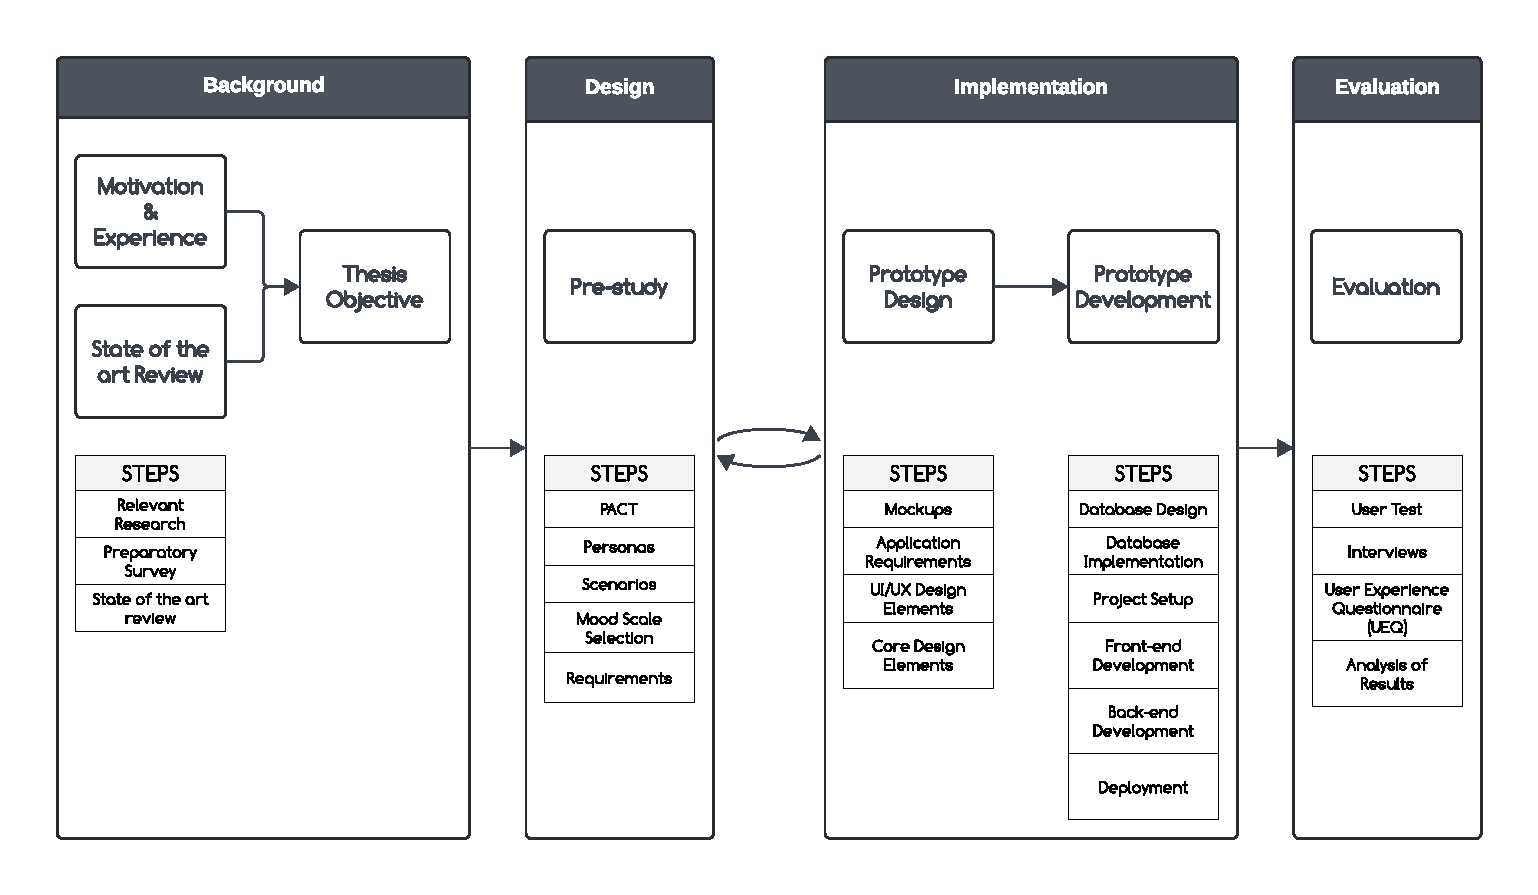
\includegraphics[width=\linewidth]{figures/Sequence-Diagram.pdf}\label{fig:sequence-diagram}
    \caption{Methodology Diagram}
\end{figure}
\FloatBarrier

\vspace{5mm}

\noindent It is important to note that the development process involved multiple iterations between the design and implementation phases. This back-and-forth approach was necessary to address various challenges that arose during implementation, such as technical limitations or usability concerns. These issues were resolved through a recurring process of redesigning and refining, ensuring that the final application aligns closely with the initial objectives and offers a seamless user experience.